\documentclass[10pt]{beamer}

%STANDARD PREAMBLE
%https://tex.stackexchange.com/questions/68821/is-it-possible-to-create-a-latex-preamble-header
\usepackage{/Users/mwojno01/Repos/latex_preamble/beamer_preamble}

%
%% ALLOW FOR ITEMIZE ENVIRONMENTS WITH NO PRECEDING
% SPACING, IF DESIRED
% Reference: https://tex.stackexchange.com/questions/86054/how-to-remove-the-whitespace-before-itemize-enumerate
%\usepackage{enumitem}% http://ctan.org/pkg/enumitem 
\usepackage{paralist}

\title{Measure-theoretic Probability}

\begin{document}

\maketitle

%\begin{frame}{Table of contents}
%  \setbeamertemplate{section in toc}[sections numbered]
%  \tableofcontents[hideallsubsections]
%\end{frame}

\begin{frame}[standout]
This slide deck is a WIP.
\vfill
(It is not complete.  Just gradually adding to it here and there.)
\end{frame}

\begin{frame}{Conditional probability}
\begin{sblock}{Elementary definition}

\begin{align*}
P(B \cond A) &= \df{P(A \cap B)}{\labeledredmathbox{what if = 0?}{P(B)}} 	
\end{align*}
\end{sblock}

\begin{sblock}{General definition}
\[ P(A \cap B)  = \int_A \labeledgreenmathbox{defined as $P(B \cond x)$}{g(x)} dP(x) \]

\begin{columns}

\begin{column}{0.45\textwidth}
\begin{figure}
\centering 
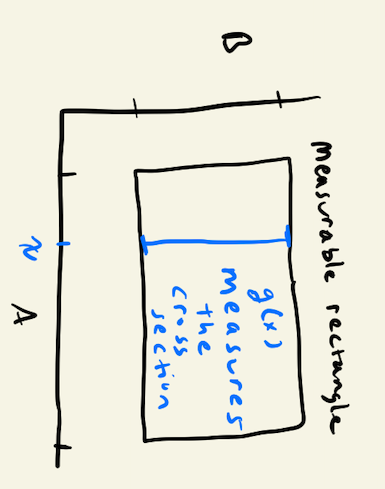
\includegraphics[angle=90,width=.7\textwidth]{images/conditional_probability_exists.png}	
\end{figure}
\end{column}

\begin{column}{0.5\textwidth}
{\scriptsize 
\textbf{Details}
\begin{itemize}
\item $\lambda(A):=P(A \cap B)$ is a finite measure on $A$. \quad Why? % Obviously finite, can show countable additivity. 
\item $\lambda \ll P$ (i.e. $P(A) = 0 \implies \lambda(A)=0$).  \quad Why?  % By monotonicity.
\item Hence $g(x)$ must exist. \quad Why?	% By Radon-Nikodym.
\end{itemize}
}
\end{column} 


\end{columns} 
\end{sblock}

	
\end{frame}



\end{document}